\documentclass[a4paper]{article}
\usepackage[utf8]{inputenc}
\usepackage{fancyhdr}
\usepackage{geometry}
\usepackage{listings}
\usepackage{graphicx}
%\geometry{0.5in}

\usepackage{float}

\lstset{
    breaklines=true,
    numbers=left,
    frame=lines
}

\pagestyle{fancyplain}

\title{System Maintenance}
\author{Harry Milne}
\date{March 2014}

\lhead{Harry Milne}
\chead{Candidate Number: 00000}
\rhead{Centre Number: 22169}

\begin{document}
\newpage
\tableofcontents

\maketitle

\section{Environment}
\label{sec:env}
\subsection{Software}
\begin{itemize}
    \item Python 2.7 and included modules
    
    \begin{itemize}
        \item SQLite3
    \end{itemize}
    
    \item Twisted 13.2.0 Python Module
    \item PyQt4 Python Module
    \item SimpleCV 1.3
    \item SQLite Database Browser
    \item Vim
    \item Sublime Text 3
\end{itemize}

\begin{table}[H]
    \centering
    \begin{tabular}{|p{4cm}|p{8cm}|}
    \hline
    Software                & Usage Explanation                                                                                                                                                                                            \\ \hline
    Python 2.7              & I used Python 2.7 instead of Python 3.* because of the superior module support that Python 2.5+ has. Also, the nature of Python itself makes it very easy to build systems quickly.                          \\ \hline
    SQLite3                 & SQLite3 was an easy database management system to use because it has little requirements for the system it is run on. This means you do not have to do any extensive configuration of any target system.      \\ \hline
    Twisted 13.2.0          & Twisted is a Python module which lets you very quickly prototype and build clients and servers, which is central to this system.                                                                             \\ \hline
    PyQt4                   & PyQt4 is a feature rich user interface development module, it handles all of the threading needed to run operations while keeping an operational interface.                                                  \\ \hline
    SimpleCV 1.3            & SimpleCV is aimed at making computer vision easy to develop, I used it in conjunction with the Raspberry Pi to recognise faces.                                                                              \\ \hline
    SQLite Database Browser & This open source software gives an easy way to visually check over your SQLite databases, this was invaluable in testing.                                                                                    \\ \hline
    Vim                     & When developing the python server script, it was easier to program it while on the server itself instead of deploying to it every time I wanted to test. This meant using a text editor that works in shell. \\ \hline
    Sublime Text 3          & This was the editor of choice while programming in a GUI environment, it has a lot of tools to help with syntax highlighting and variable naming.                                                            \\ \hline
    \end{tabular}
\end{table}

\section{System Overview}
The system has 3 main components; the client, server and database browser. The server and client are directly related
whereas the database browser is a `tool' I have bundled to help the user manage the database. The database browser works
with the server on a local level, in that you edit the same file on the same system that the server does. However,
the database browser requires the server to be running a graphical user environment because it is a graphical representation
of the database. 

\subsection{Client}
The client uses the SimpleCV package as shown in section~\ref{sec:env}, this package handles everything around the camera,
this makes it easier to read what is happening with the data being handled by the Python.  

\subsection{Server}


\subsection{Database Browser}

\section{Code Structure}
I structured the code so that each section of the system was an object, abstracting like this helps a lot with
visualising the code. By doing this I have taken one of the advantage of object-oriented programming; the ability
to abstract certain situations into particular `objects'.

\subsection{Particular Code Section}
\section{Variable Listing}
\section{System Evidence}
\subsection{User Interface}
\subsection{ER Diagram}
\begin{center}
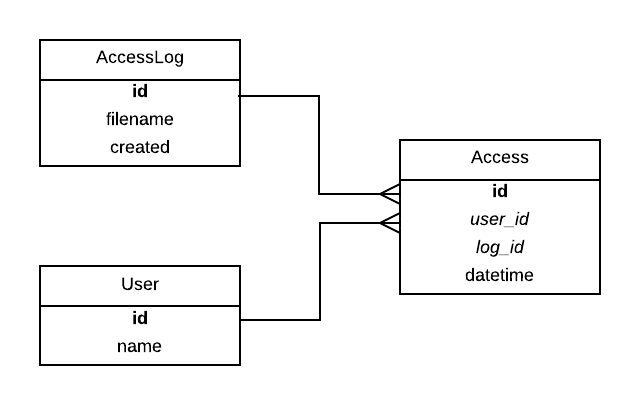
\includegraphics[scale=0.6]{../shared_assets/diagrams/ERD.png}
\end{center}
\subsection{Database Table Views}
\subsection{Database SQL}
\subsection{SQL Queries}
\section{Testing}
\subsection{Summary of Results}
\subsection{Known Issues}
\section{Code Explanations}
\subsection{Difficult Sections}
\begin{itemize}
    \item Learning SimpleCV
    \item Learning Twisted
    \item Handling Physical Log Files
    \item Editing an existing project
\end{itemize}
\subsection{Self-created Algorithms}
\section{Settings}
\subsection{Server}
The server has it's settings contained in a `.cfg' file, which is placed in the same directory as `main.py',
the system uses a Python object called `ConfigParser' which reads from this plain-text file and stores it in
the object.
\lstinputlisting[caption=server.cfg]{../../code/server/server.cfg}

\subsection{Client}
\ref{sec:client.py}
%\lstinputlisting{../../code/client/client.cfg}
\section{Acknowledgements}
\subsection{Adam McNicol}
The code I used to create the Database Browser was forked from the repository from github.com/MrAGi, I trimmed
down the original code and edited things like the file browser to more suit my needs. Taking advantage of
open source projects is a great way of saving time and learning from other peoples code. After seeing the code
in use before, it seemed logical to just take that project and change it slightly to fit my project. The best
thing about it was that it was already very well tested since the entire class had already been using it without
any problems.

\subsection{Code Listing Appendix}
\newpage
\subsubsection{client/client.py}
\label{sec:client.py}
\lstinputlisting{../../code/client/client.py}

\subsubsection{server/main.py}
\label{sec:main.py}
\lstinputlisting{../../code/server/main.py}

\subsubsection{server/server.py}
\label{sec:server.py}
\lstinputlisting{../../code/server/server.py}

\subsubsection{server/sql\_interface.py}
\label{sec:sqlinterface.py}
\lstinputlisting{../../code/server/sql_interface.py}

\subsubsection{db\_browser/db\_browser.pyw}
\label{sec:dbbrowser.py}
\lstinputlisting{../../code/db_browser/db_browser.pyw}

\subsubsection{db\_browser/dialogs.py}
\label{sec:dialogs.py}
\lstinputlisting{../../code/db_browser/dialogs.py}

\subsubsection{db\_browser/sqlite\_browse\_data.py}
\label{sec:browsedata.py}
\lstinputlisting{../../code/db_browser/sqlite_browse_data.py}

\subsubsection{db\_browser/sqlite\_connection.py}
\label{sec:connection.py}
\lstinputlisting{../../code/db_browser/sqlite_connection.py}


\end{document}
